\documentclass[BIND,norsk,twoside]{gucthesis}


% PACKAGES %
\usepackage[utf8x]{inputenc}     % For utf8 encoded .tex files
\usepackage[pdftex]{graphicx, hyperref}   % For cross references in pdf
\usepackage{float}
\usepackage{color}              % For colouring text   
\usepackage{nomencl}    % For abbreviation
\usepackage{pdfpages}
\usepackage{longtable}
\usepackage[table,tabulator]{xcolor}
\makenomenclature       % Use with \nomenclature{Abbreviation}{Full text}
            % Compile with: "makeindex main.nlo -s nomencl.ist -o main.nls"
            % Before and after latex of pdflatex

% Definitions of colors for use in document
\definecolor{lightgray}{gray}{0.9}
\definecolor{darkgray}{gray}{0.8}

% COMMENTS AND NOTES %
\newcommand{\comment}[1]{\textcolor{blue}{\emph{#1}}}  %% use of the colour and you can see how to use commands with parts \comment{so what}
\newcommand{\com}[1]{{\color{red}#1}} % supervisor comment
\newcommand{\todo}[1]{{\color{green}#1}} % items to do
\newcommand{\n}[1]{{\color{blue}#1}} % other comment
\newcommand{\dn}[1]{} % add the d to a note to say that you have finished with it.
\renewcommand{\nomname}{List of Abbreviations}
\newcommand{\tab}{\hspace*{2em}} % aligning the text as one tab stop

\begin{document}

\thesistitle{SkyHiGh Feide}
\thesisauthor{Fredrik Magnussen}
\thesisauthorA{Håkon Tvedt}
\thesisauthorB{Morten H. Singstad}
%\thesisauthorC{}
\thesissupervisor{Hanno Lagweg}
%\thesissupervisorA{} %second supervisor

\gmtkeywords{Thesis, Latex, Template, IMT}
\gmtdesc{This is the short description of a bachelor thesis}
\gmtnumber{-} % this is the number given to your project. May not be used  

\gmtoppdragsgiver{Erik Hjelmås, Høgskolen i Gjøvik}
\gmtcontact{Erik Hjelmås, erikh@hig.no}




\thesisdate{\gucthesisdate}
\useyear{15.05.2013}

\gmtappnumber{} %numebr of appendixes
\gmtpagecount{} %currently auto calculated but might be wrong


\thesistitleNOR{Norwegian title.}
\gmtkeywordsNOR{Norway, Norsk}
\gmtdescNOR{This should be in Norwegian, I thought I would add some more text
to make sure that it ran over multiple lines. I will need to check the page
number feild as it probably should be just the core pages without the
appendices.  Currently it returns the last page of the whole document. 
If I cannot work it out, I will provide two inputs, gmtnumberpages and gmtappnumber.
That should do the job.}

 % this is the file which contains all the details about your thesis

\makefrontpages

%\input{chapters/forord}

\tableofcontents
\vfill \hfill \textbf{Word count: 123} % Requirement according to the template
                                       % to print word count without appendix
\listoffigures
\listoftables
\printnomenclature

%\input{chapters/innholdsfortegnelse}
\begin{center}
	\chapter{Innledning}
\end{center}
\section{Bakgrunn}
Autentisering, er i dag et stort tema. Det er mye snakk på at det blir for mange brukernavn og passord å huske. Det diskuteres også at dette skader sikkerheten av data. Grunnen til dette er at brukerne lager seg lettere passord, lagrer passord på telefonen, post-it-lapper og mange andre finurlige måter. Dette er ingen heldig situasjon, men det er veldig forståelig at det blir sånn. \newline \newline
En av løsningene på dette er FEIDE\cite{Omfeide}. Denne løsningen er kunnskapsdepartementets svar på problemet. Denne løsningen er kun innenfor utdanningssektoren i Norge, men det vil være en stor reduksjon i hvor mange brukernavn og passord som må huskes. \newline \newline
Det er derfor blitt et ønske fra Erik Hjelmås fra Høgskolen i Gjøvik å integrere dette på skyløsningen til skolen. Openstack-skyløsningen ved HiG skal i første omgang være tilgjengelig for ansatte og fag. Det er flere fag som bruker VM-er i undervisningen (Ethical Hacking And Penetration Testing \cite{imt3491}, Systemadministrasjon \cite{imt3292} og Database- og applikasjonsdrift \cite{imt3441}). \newline \newline
\textbf{Ønsker fra arbeidsgiver}
\begin{description}
	\item[\tab •] Sentral innlogging for VM-er.
	\item[\tab •] Skal kunne bruke brukernavn og passord som man har ellers på skolen.
\end{description}
Nåværende løsning er at det står to servere som har lokale brukere. Disse opprettes om vedlikeholdes i passwd- og shadowfilene. Dette er en tungvint løsning ved når man ønsker å utvide VM-systeme for bruk av flere ved HiG.

\newpage
\section{Oppgavebeskrivelse}
Hensikten ved bacheloroppgaven SkyHiGhFeide er at vi skal integrere modul i Openstack som autentiserer mot Feide (Openstack er et “open source cloud computing”-prosjekt). Denne løsning vil gjøre at man kan bruke allerede brukernavn og passord som man har i Feide. Flere tjenester i undervisningssektoren i Norge bruker Feide, målet til kunnskapsdepartemnetet er at alt innen skole-Norge skal autentiseres mot Feide. Ved denne modul-integreringen i Openstack vil det da bli en standard i innlogging. \newline \newline
Vi skal sette opp et rack med Openstack-løsning som skal kjøre VM-systemet for skolen. Dette vil bedre ytelse og effektiviteten ved bruk av VM på HiG. Vi skal sette opp autentiseringen mot horizon-platformen på kontrollernoden i Openstack. Denne skal kjøre autentisering mot keystone-platformen i Openstack, som er autentiseringstjenesten i Openstack. 
\begin{description}
\item[\tab •] Sette opp SkyHiGh løsningen og oppdatere denne til siste versjon av OpenStack.
\item[\tab •] Utrede og realisere rollebasert identitetshåndtering og tilhørende FEIDE-autentisering.
\end{description}
\section{Rapportorganisering}
\begin{description}
\item[\tab 1.] Innledning - Et lite innblikk i rapporten. Gir en kort overordnet oversikt av hvordan rapporten er strukturert og hva den inneholder.
\item[\tab 2.] Kravspesifikasjon - Her dokumenteres kravene som arbeidsgiver har satt for hvordan systemet skal fungere med autentisering mot Openstack.
\item[\tab 3.] Teoretisk grunnlag Openstack - Her gir en grundig inføring i hvordan autentiseringen fungerer i Openstack. Dette er viktig for å få forståelse for hvor og hvordan vi skal kunne integrere Feide-autentisering.
\item[\tab 4.] Teoretisk grunnlag Feide - Her gir vi en grundig inføring og forklaring av hvordan Feide-autentisering fungerer. Veldig viktig for forståelse av hvordan vi skal kunne autentisere mot Openstack.
\item[\tab 5.] Design - Går mer inn på designet autentiseringen i Openstack og Feide, samt detaljert design som er utbedret av kravspesifikasjonen.
\item[\tab 6.] Gjennomføring - Her vil det bli detaljert, dokumentert og godt beskrivende forklaring på hvordan vi gjennomfører prosjektet. 
\item[\tab 7.] Driftrutiner - Her gir vi en forklaring på hvordan det skal vedlikeholdes og oppdateres for å opprettholde sikkerhet og brukervennlighet.
\item[\tab 8.] Drøting - Vi diskuterer om det finnes andre og kanskje bedre muligheter i forhold til autentisering. Litt nøyere drøfting det vi har gjort kontra andre. Spør oss selv om sikkerheten blir svekket. 
\item[\tab 9.] Avlsuttning - Konklusjonen fra oppgaven, hvordan resultatet ble og hvordan utførelsen ble gjort.
\item[\tab 10.] Bibliografi og litteraturliste - En oversikt over referanser og tekster som er brukt i denne rapporten, samt en liste over komplekse ord.
\item[\tab 11.] Vedlegg - Dokumentering av figurer, tabeller til rapporten. Andre vedlegg: Prosjektplan, script, dagslogg og referater fra diverse møter.
\end{description}

\newpage
\section{Beskrivelser}
Her kommer noen regler og beskrivelser på hvordan spesielle ord brukes i rapport og blir forklart. \newline \newline
Vi-ordet refereres til prosjektgruppen vår som består av Fredrik Magnussen, Håkon Tvedt og Morten H. Singstad. Når vi snakker om arbeidsgiver, er det Erik Hjelmås. Hanno Langweg refereres som veileder.
\begin{description}
\item[\tab •] Forkortelser vil bli beskrevet i sitt fulle navn i fotnoten.
\item[\tab •] Andre spesielle ord vil få et eksponentnummer som kan refereres til litteraturlisten.
\item[\tab •] Kommandoer og script vil ha denne fonten ved navn Courier new, på scriptene vil det også være syntax-farger.
\item[\tab •] For kildehenvisning benytter vi oss av vancouver-stilen \cite{vancouver}
\item[\tab •] Ord som er relevant å forklare i teksten vil ikke bli nevnt i litteraturlisten.
\end{description}

\section{Formål}
Formålet med å integrere FEIDE-autentisering i Openstack vil være en forenklet hverdag for brukerne av SkyHiGh\cite{skyhigh}, ved at de kan logge inn med brukernavn og passord som de har fra før. Det skal være rollebasert innlogging. Da mener vi at det skal være forskjellige rettigheter hvis en ansatt logger inn kontra en student. Det viktigste er at det funker ved HiG, men hvis mulig skal vi lage en integrering som skal kunne brukes for andre Openstack-brukere. Dagens innlogging består av to servere som lagrer nye brukernavn og passord i passwd- og shadow-filene. Ugunstig ved at man må legge til nye brukere for hvert semester samt slette de gamle. 
\newline \newline
Formålet skal også være å øke sikkerheten. Ved at brukerne får enda et nytt brukernavn og passord å huske, så er det stor sannsynlighet at brukerne skriver ned passordet på mobil, post-it-lapp eller andre steder som svekker sikkerheten. Ved at man kan bruke brukernavn og passord som brukerne har fra før, så trenger man ikke huske nye data, samt at det er større sannsynlighet for at brukerne ikke trenger å skrive informasjonen ned.

\section{Målgruppe}
\subsection{Prosjektets målgruppe}
Målgruppen for prosjektet er HiG. Det skal være en løsning som først og fremst er rettet for å fungere her. I første omgang for de ansatte med fagene som krever VM-er, deretter for alle ansatte ved skolen. Hvis en framtidig utvidelse av SkyHiGh skulle komme, så er det ønskelig at løsningen skal være tigjengelig for enkeltstudenter.
\subsection{Rapportens målgruppe}
Rapporten er myntet på at det skal være dokumentert utførelse av prosjektet til arbeidsgiver. Derav skal det være mulig for andre interesserte å kunne se hva vi har gjort, for så å kunne integrere løsningen selv hvis ønskelig. Rapporten er også i hovedsak en utdanning. For oss som gruppe, så er dette en erfaring vi kan bringe med oss videre inn i arbeidslivet.
\section{Avgrensning}
Hovedmålet for oppgaven er at det skal være fungerende innlogging til Openstack mot Feide. Nødløsning er at vi får en løsning som kun fungerer for denne skolen gjennom å autentisere med LDAP-registeret til skolen. Dokumentasjon for dette vil også vedvare for at andre interessenter skal kunne bruke nødløsningen hvis de selv bruker LDAP. Siden vi er drift-studenter, ser vi det også vesentlig at vi automatiserer det som kan automatiseres. \newline \newline
Deretter så er det tid som avgrenser hva vi får gjort. Ønsket er å få satt opp et rack med kjørende Openstack-løsning med integrert Feide-autentisering. Bonusmål: Overvåking og implementering av SkyHiGh Adm-modulen.

\section{Prosjektgruppens kunnskap}
Prosjektgruppens faglige bakgrunn er den samme. Fredrik Magnussen, Håkon Tvedt og Morten H. Singstad går alle tre “Drift av nettverk- og datasystemer” ved HiG. Vi har brukt VM-er i fag og lært hvordan de blir opprettes, samt hvordan de oppererer på en maskin. Men kunnskap i hvordan Openstack-løsningen fungerer er heller liten. Heller ikke autentisering i seg selv har vi noen faglige kunnskaper ved.\newline \newline
Det vi har av faglige kunnskaper som kan hjelpe oss er grunnforståelse og god teknisk innsikt. Programmeringskunnskapen vi har opparbeidet oss her på skolen vil også komme godt til nytte med tanke på script. Scriptene vil i all hovedsak lages for å automatisere installasjonen av Openstack, som er drøftet i Vedlegg A. \newline \newline
Vi er derfor nødt til å tilegne oss mye kunnskap fra bunnen av. Innenfor Feide, Openstack og nye programeringsspråk. Vi er nødt til å sette oss grundig inn i hvordan Openstack autentiserer brukerne sine.

\section{Roller}
Arbeidsgiveren våres er Erik Hjelmås, ansatt ved HiG som førsteamanuensis. Kunnskapen til arbeidsgiver angående Feide vil ikke kunne være noen stor ressurs. Men erfaringsmessig kan han bidra oss med å lete på rett plass og stille de rette spørsmålene for å kunne få den kunnskapen vi trenger. Arbeidgiver er også en stor ressurs ved materialistiske behov. \newline \newline
Veileder Hanno Langweg som også er ansatt ved HiG som førsteamanuensis, kommer til å være en sterk ressurs innenfor hvordan prosjektet bør gjennomføres. Bidrag med hvordan vi bør prioritere i et så stor prosjekt og hjelpe oss med å nå de målene vi har satt oss. \newline \newline
Rolleinndeling under prosjektarbeidet:
\begin{description}
\item[\tab •] Morten H. Singstad \\ Valgt som leder for prosjektgruppa. Vil være den som er kontaktperson og som har det overordna ansvaret for gruppen og oppgavene.
\item[\tab •] Fredrik Magnussen \\ Webansvarlig.
\item[\tab •] Håkon Tvedt \\ Ansvaret for alt som har med installasjoner.
\end{description}
Når alt kommer til alt, så er vi en samarbeidende prosjektgruppe som hjelper hverandre og er ydmyke i rollene. Vi er bestemte, men har ingen ovenfra-og-ned-holdning ovenfor hverandre.
%\clearpage
\chapter{Kravspesifikasjon}
Vi skal få inn en tjeneste under et allerede eksisterende rammeverk. Med det må vi beskrive de kravene som må opprettholdes for at vi skal kunne få en suksessfull integrering med ny autentisering. Vi skal også beskrive detaljert hendelsesløpet for en autentisering innenfor rammeverket, eksisterende og det vi vil integrere. \newline \newline
Allerede eksisterende materiale vi kan se på er dokumentasjon på Openstack keystone-modulen og Feide-dokumentasjon.

\section{Brukerbeskrivelse}
\subsection{Omgivelser}
Som nevnt tidligere, så skal autentiseringstjenesten integreres. Det skal skje på et allerede eksisterende system, som allerede har en annen autentiseringstjeneste. Selve Openstack-systemet samkjøres mellom flere servere. Det er stykket opp i moduler for ytelse og funksjonalitet. Den modulen vi skal jobbe på er “Controller noden”, den kjører noen moduler som vi skal jobbe med og derfor må sette oss ekstra nøye inn i.

\begin{description}
	\item{\tab •} Horizon - Webinterfacet til Openstack-systemet. Der er brukergrensesnittet som brukes for å kunne lage, endre, slette og kjøre VM-ene, det er også her innloggingen ligger.
	\item{\tab •} Keystone - Tar seg av hvilke prosesser og VM-er som tilhører hvem. Derfor har også den en finger med i autentiseringen.
\end{description}

\subsection{Systemets brukere}
Det er tre grupper med brukere mot tjenesten vi skal integrere. De har alle forskjellige roller og autoritet innen systemet.

\begin{description}
	\item{\tab •} Studenter/brukere - De har kun lov til å kunne lage, endre, slette og bruke VM-er. De har også restriksjoner på ytelse og mengde plass som kan brukes.
	\item{\tab •} Ansatte - Forskjellen fra studentene er at de ansatte har ikke restriksjon på ytelse og mengde data.
	\item{\tab •} It-tjenesten - Gruppen som har mest tilgang, men av den praktiske grunn at de har vedlikeholdsarbeidet. De har også rettigheter som de overnevnte.
\end{description}

Opplæringen ved å bruke tjenesten er minimal. Vi skal jobbe med innloggingen. Noe absolutt alle har vært borti før, med tanke på at det er noe av det første du må gjøre når du kommer til HiG.

\newpage
\subsection{User stories}
\subsection{Primærmål}
\begin{table}[H]
	\begin{tabular}[Figur 2]{| p{2cm} p{9cm} |}
		\hline \textbf{Stikkord} & logge inn på domene \\
		\hline \textbf{Beskrivelse} & Brukeren vil at man skal kunne skrive inn et gitt domene og komme til log in-skjermen. I dette tilfelle er domene allerede ordnet: skyhigh.hig.no.
	\end{tabular}
\end{table}

\begin{table}[H]
	\begin{tabular}[Figur 2]{| p{2cm} p{9cm} |}
		\hline \textbf{Stikkord} & logge in med Feide\\
		\hline \textbf{Beskrivelse} & Kunden vil at brukeren må logge seg inn ved å bruke eksisterende brukernavn og passord. 
	\end{tabular}
\end{table}

\begin{table}[H]
	\begin{tabular}[Figur 2]{| p{2cm} p{9cm} |}
		\hline \textbf{Stikkord} & Forskjellige roller\\
		\hline \textbf{Beskrivelse} & Kunden ønsker at det skal være forskjell på hvilke roller man har når man logger in. De ansatte som trenger VM-er i undervisninger trenger gjerne litt ekstra ytelse, dette i forhold til at det kan være mange studenter i et emne og må derfor delegere ut mange VM-er. Hvis ansatte bare vil bruke et par VM-er så trenger de ikke rettigheter utover det vanlige.
		\begin{description}
			\item[Det vil bli satt opp to forskjellige roller:]
			\item[\tab •] Ekstra rettigheter
			\item[\tab •] Normal rettigheter
		\end{description}		 
	\end{tabular}
\end{table}

\subsection{Sekundærmål}
\begin{table}[H]
	\begin{tabular}[Figur 2]{| p{2cm} p{9cm} |}
		\hline \textbf{Stikkord} & Installere Openstack \\
		\hline \textbf{Beskrivelse} & Openstack skal bli HiG sin skyløsning. Skolen bruker en del VM-er og trenger mer ytelse på de. Derfor blir løsningen å sette opp eget. 
	\end{tabular}
\end{table}

\begin{table}[H]
	\begin{tabular}[Figur 2]{| p{2cm} p{9cm} |}
		\hline \textbf{Stikkord} & Installere Openstack \\
		\hline \textbf{Beskrivelse} & Openstack skal bli HiG sin skyløsning. Skolen bruker en del VM-er og trenger mer ytelse på de. Derfor blir løsningen å sette opp eget. \\
	\end{tabular}
\end{table}

\begin{table}[H]
	\begin{tabular}[Figur 2]{| p{2cm} p{9cm} |}
		\hline \textbf{Stikkord} & Installere Adm-modulen \\
		\hline \textbf{Beskrivelse} & Kunden ønsker også, hvis tid, at vi skal få installert Adm-modulen som bachelorgruppa SkyHiGh Adm lagde. 
	\end{tabular}
\end{table}

\begin{table}[H]
	\begin{tabular}[Figur 2]{| p{2cm} p{9cm} |}
		\hline \textbf{Stikkord} & Automatisert innstallasjon \\
		\hline \textbf{Beskrivelse} & Med tanke på vedlikehold så vil det være enkelt og greit med en automatisert installasjon. F.eks. hvis det blir satt inn en “Compute node” til, så skal det kun være å boote en usbpinne som tar seg av hele installasjonen.  \\
	\end{tabular}
\end{table}

\newpage
\section{Detaljert kravspesifikasjon}
\subsection{Funksjonelle krav}
Kravene for funksjonaliteten av tjenesten vil være å få opp modulen som kjører webinterfacet til SkyHiGh. Webinterfacet ligger på Controller node-en i modulen Horizon. For å kunne sette opp Controller node-en er vi nødt til å ha en server å jobbe på. Det er der login-screenet skal være. Login-screenet skal autentiseres mot Feide, det vil også si at vi er nødt til å få opp en testbruker hos Feide. Feide bruker SAML 2.0 som er et xml-basert språk for autentisering. \newline \newline
For at vi skal få autentisert med forskjellige roller må vi legge til noen ekstra metadata til SAML 2.0 dokumentet. Vi må også studere hvordan autentiseringen foregår mellom Horizon- og Keystone modulene for å kunne se hvilke data som sendes mellom de. Disse dataene trengs for å kunne konfigurere SAML 2.0 dokumentet til å ta imot de rette dataene, for dette å kunne autentiseres som forskjellige roller. Så må vi konfigurere på Horizon hvilke oppgaver som skal være tillatt for de forskjellige rollene. 
\subsection{Use case diagram}
\begin{figure}[H]
      \center{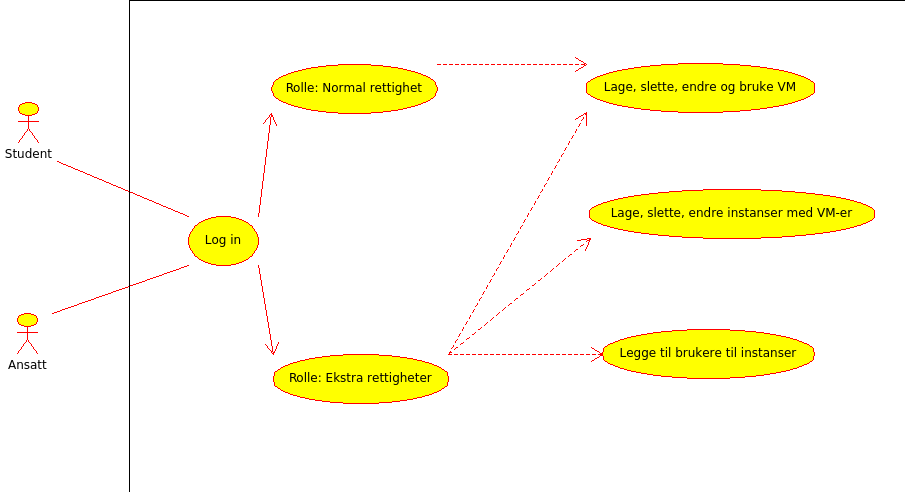
\includegraphics[width=100mm,height=90mm]{bilder/use_case_diagram}}
      \caption{\label{fig:usecase} Use case diagram 1}
\end{figure}

\begin{figure}[H]
	\center{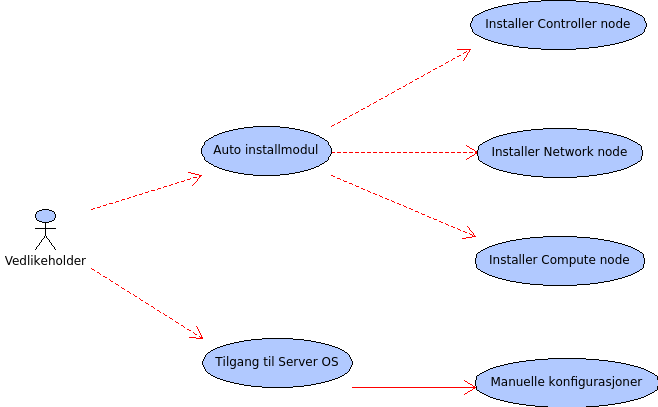
\includegraphics[width=100mm,height=90mm]{bilder/use_case_diagram_2}}
    \caption{\label{fig:usecase2} Use case diagram 2}
\end{figure}

\clearpage
\subsection{Høynivå use case}
\begin{table}[H]
	\begin{tabular}[Figur 1]{| p{1cm} | p{3cm} | p{3cm} | p{3cm} | p{2cm} }
		\hline \rowcolor{lightgray} \textbf{Use case ID} & \textbf{Usecase-navn} & \textbf{aktør} & \textbf{Kompleksitet} & \textbf{Prioritet} \\
		\hline \rowcolor{darkgray} 1 & Log in & Student og ansatt & Høy & 1 \\
		\hline \rowcolor{lightgray} 2 & Rolle: Normal rettighet & Student og ansatt & Middels & 2 \\
		\hline \rowcolor{darkgray} 3 & Rolle: Ekstra rettighet & Noen ansatte & Middels & 2 \\
		\hline \rowcolor{lightgray} 4 & Konfigurere VM-er & Lav & Studenter og ansatte & 2 \\
		\hline \rowcolor{darkgray} 5 & Konfigurere VM-instanser & Noen ansatte & Lav & 2 \\
		\hline \rowcolor{lightgray} 6 & Administrere VM-instanser & Noen ansatte & Middels & 3 \\
		\hline \rowcolor{darkgray} 7 & Auto install-modul & Vedlikeholder & Lav & 3 \\
		\hline \rowcolor{lightgray} 8 & Installer Controller node & Vedlikeholder & Lav & 3 \\
		\hline \rowcolor{darkgray} 9 & Installer Network node & Vedlikeholder & Lav & 3 \\
		\hline \rowcolor{lightgray} 10 & Installer Compute node & Vedlikeholder & Lav & 3 \\
		\hline \rowcolor{darkgray} 11 & Tilgang til server-OS & Vedlikeholder & Lav & 3 \\
		\hline \rowcolor{lightgray} 12 & Manuelle konfigurasjoner & Vedlikeholder & Lav & 3 \\
		\hline
	\end{tabular}
\end{table}

\begin{table}[H]
	\begin{tabular}[Figur 2]{| p{2cm} | p{9cm} |}
		\hline \rowcolor{lightgray} \textbf{Use case ID} & 1 \\
		\hline \rowcolor{darkgray} \textbf{Use case navn} & Log in \\
		\hline \rowcolor{lightgray} \textbf{aktør} & Ansatt og student\\
		\hline \rowcolor{darkgray} \textbf{Beskrivelse} & En bruker prøver å logge seg inn på SkyHiGh. Denne tar imot brukernavn og passord, samt innformasjon om fylke. \\
		\hline
	\end{tabular}
\end{table}

\begin{table}[H]
	\begin{tabular}[Figur 3]{| p{2cm} | p{9cm} |}
		\hline \rowcolor{lightgray} \textbf{Use case ID} & 2 \\
		\hline \rowcolor{darkgray} \textbf{Use case navn} & Rolle: Normal rettighet \\
		\hline \rowcolor{darkgray} \textbf{aktør} & Ansatt og student\\
		\hline \rowcolor{lightgray} \textbf{Beskrivelse} & Med innloggingsinformasjonen til brukeren vil autentiseringsprosessen avgjøre hvilke rettigheter brukeren har. \\
		\hline
	\end{tabular}
\end{table}

\begin{table}[H]
	\begin{tabular}[Figur 4]{| p{2cm} | p{9cm} |}
		\hline \rowcolor{lightgray} \textbf{Use case ID} & 3 \\
		\hline \rowcolor{darkgray} \textbf{Use case navn} & Rolle: Ekstra rettigheter \\
		\hline \rowcolor{lightgray} \textbf{aktør} & Noen ansatte\\
		\hline \rowcolor{darkgray} \textbf{Beskrivelse} & Med innloggingsinformasjonen til brukeren vil autentiseringsprosessen avgjøre hvilke rettigheter brukeren har. \\
		\hline
	\end{tabular}
\end{table}

\begin{table}[H]
	\begin{tabular}[Figur 5]{| p{2cm} | p{9cm} |}
		\hline \rowcolor{lightgray} \textbf{Use case ID} & 4 \\
		\hline \rowcolor{darkgray} \textbf{Use case navn} & Konfigurere VM-er \\
		\hline \rowcolor{lightgray} \textbf{aktør} & Ansatt og student\\
		\hline \rowcolor{darkgray} \textbf{Beskrivelse} & Her kan de brukeren lage, endre, slette og bruke VM-er. Her er det restriksjoner på ytelse og menge plass utifra hvilken rettighet brukeren har. \\
		\hline
	\end{tabular}
\end{table}

\begin{table}[H]
	\begin{tabular}[Figur 6]{| p{2cm} | p{9cm} |}
		\hline \rowcolor{lightgray} \textbf{Use case ID} & 5 \\
		\hline \rowcolor{darkgray} \textbf{Use case navn} & Konfigurere instanser med VM-er \\
		\hline \rowcolor{lightgray} \textbf{aktør} & Noen ansatte\\
		\hline \rowcolor{darkgray} \textbf{Beskrivelse} & Brukeren kan lage, endre, slette og bruke instanser med VM-er. \\
		\hline
	\end{tabular}
\end{table}

\begin{table}[H]
	\begin{tabular}[Figur 7]{| p{2cm} | p{9cm} |}
		\hline \rowcolor{lightgray} \textbf{Use case ID} & 6 \\
		\hline \rowcolor{darkgray} \textbf{Use case navn} & Administrere VM-instanser \\
		\hline \rowcolor{lightgray} \textbf{aktør} & Noen ansatte\\
		\hline \rowcolor{darkgray} \textbf{Beskrivelse} & Her har brukeren lov til å administrere de forskjellige instansene med VM-er. \\
		\hline
	\end{tabular}
\end{table}

\begin{table}[H]
	\begin{tabular}[Figur 2]{| p{2cm} | p{9cm} |}
		\hline \rowcolor{lightgray} \textbf{Use case ID} & 7 \\
		\hline \rowcolor{darkgray} \textbf{Use case navn} & Auto installmodul \\
		\hline \rowcolor{lightgray} \textbf{aktør} & Vedlikeholder\\
		\hline \rowcolor{darkgray} \textbf{Beskrivelse} & Denne modulen består enten at installerings-scriptet blir hentet fra en server, eller så er det en usbpinne som har tre forskjellige installeringer. Da er det bare å velge rett installering til rett modul i Openstack man skal installere. \\
		\hline
	\end{tabular}
\end{table}

\begin{table}[H]
	\begin{tabular}[Figur 2]{| p{2cm} | p{9cm} |}
		\hline \rowcolor{lightgray} \textbf{Use case ID} & 8 \\
		\hline \rowcolor{darkgray} \textbf{Use case navn} & Installer Controller node \\
		\hline \rowcolor{lightgray} \textbf{aktør} & Vedlikeholder \\
		\hline \rowcolor{darkgray} \textbf{Beskrivelse} & Script som kjører installasjonen av Controller noden. \\ 
		\hline
	\end{tabular}
\end{table}

\begin{table}[H]
	\begin{tabular}[Figur 2]{| p{2cm} | p{9cm} |}
		\hline \rowcolor{lightgray} \textbf{Use case ID} & 9 \\
		\hline \rowcolor{darkgray} \textbf{Use case navn} & Installer Network node\\
		\hline \rowcolor{lightgray} \textbf{aktør} & Vedlikeholder \\
		\hline \rowcolor{darkgray} \textbf{Beskrivelse} & Script som kjører installasjonen av Network noden. \\
		\hline	
	\end{tabular}
\end{table}

\begin{table}[H]
	\begin{tabular}[Figur 2]{| p{2cm} | p{9cm} |}
		\hline \rowcolor{lightgray} \textbf{Use case ID} & 10 \\
		\hline \rowcolor{darkgray} \textbf{Use case navn} & Installer Compute node \\
		\hline \rowcolor{lightgray} \textbf{aktør} & Vedlikeholder \\
		\hline \rowcolor{darkgray} \textbf{Beskrivelse} & Script som kjører installasjonen av Commpute noden. \\
		\hline	
	\end{tabular}
\end{table}

\begin{table}[H]
	\begin{tabular}[Figur 2]{| p{2cm} | p{9cm} |}
		\hline \rowcolor{lightgray} \textbf{Use case ID} & 11 \\
		\hline \rowcolor{darkgray} \textbf{Use case navn} & Tilgang til server-OS-et \\
		\hline \rowcolor{lightgray} \textbf{aktør} & Vedlikeholder \\
		\hline \rowcolor{darkgray} \textbf{Beskrivelse} & Dette er direkte tilgang til serverne. \\
		\hline
	\end{tabular}
\end{table}

\begin{table}[H]
	\begin{tabular}[Figur 2]{| p{2cm} | p{9cm} |}
		\hline \rowcolor{lightgray} \textbf{Use case ID} & 12 \\
		\hline \rowcolor{darkgray} \textbf{Use case navn} & Manuell konfigurasjon \\
		\hline \rowcolor{lightgray} \textbf{aktør} & Vedlikeholder \\
		\hline \rowcolor{darkgray} \textbf{Beskrivelse} & Dette er hvis vedlikeholder trenger å installere noe mer på serveren eller konfigurere noe. \\
		\hline
	\end{tabular}
\end{table}
\subsection{Detaljert use case}
\begin{figure}[H]
	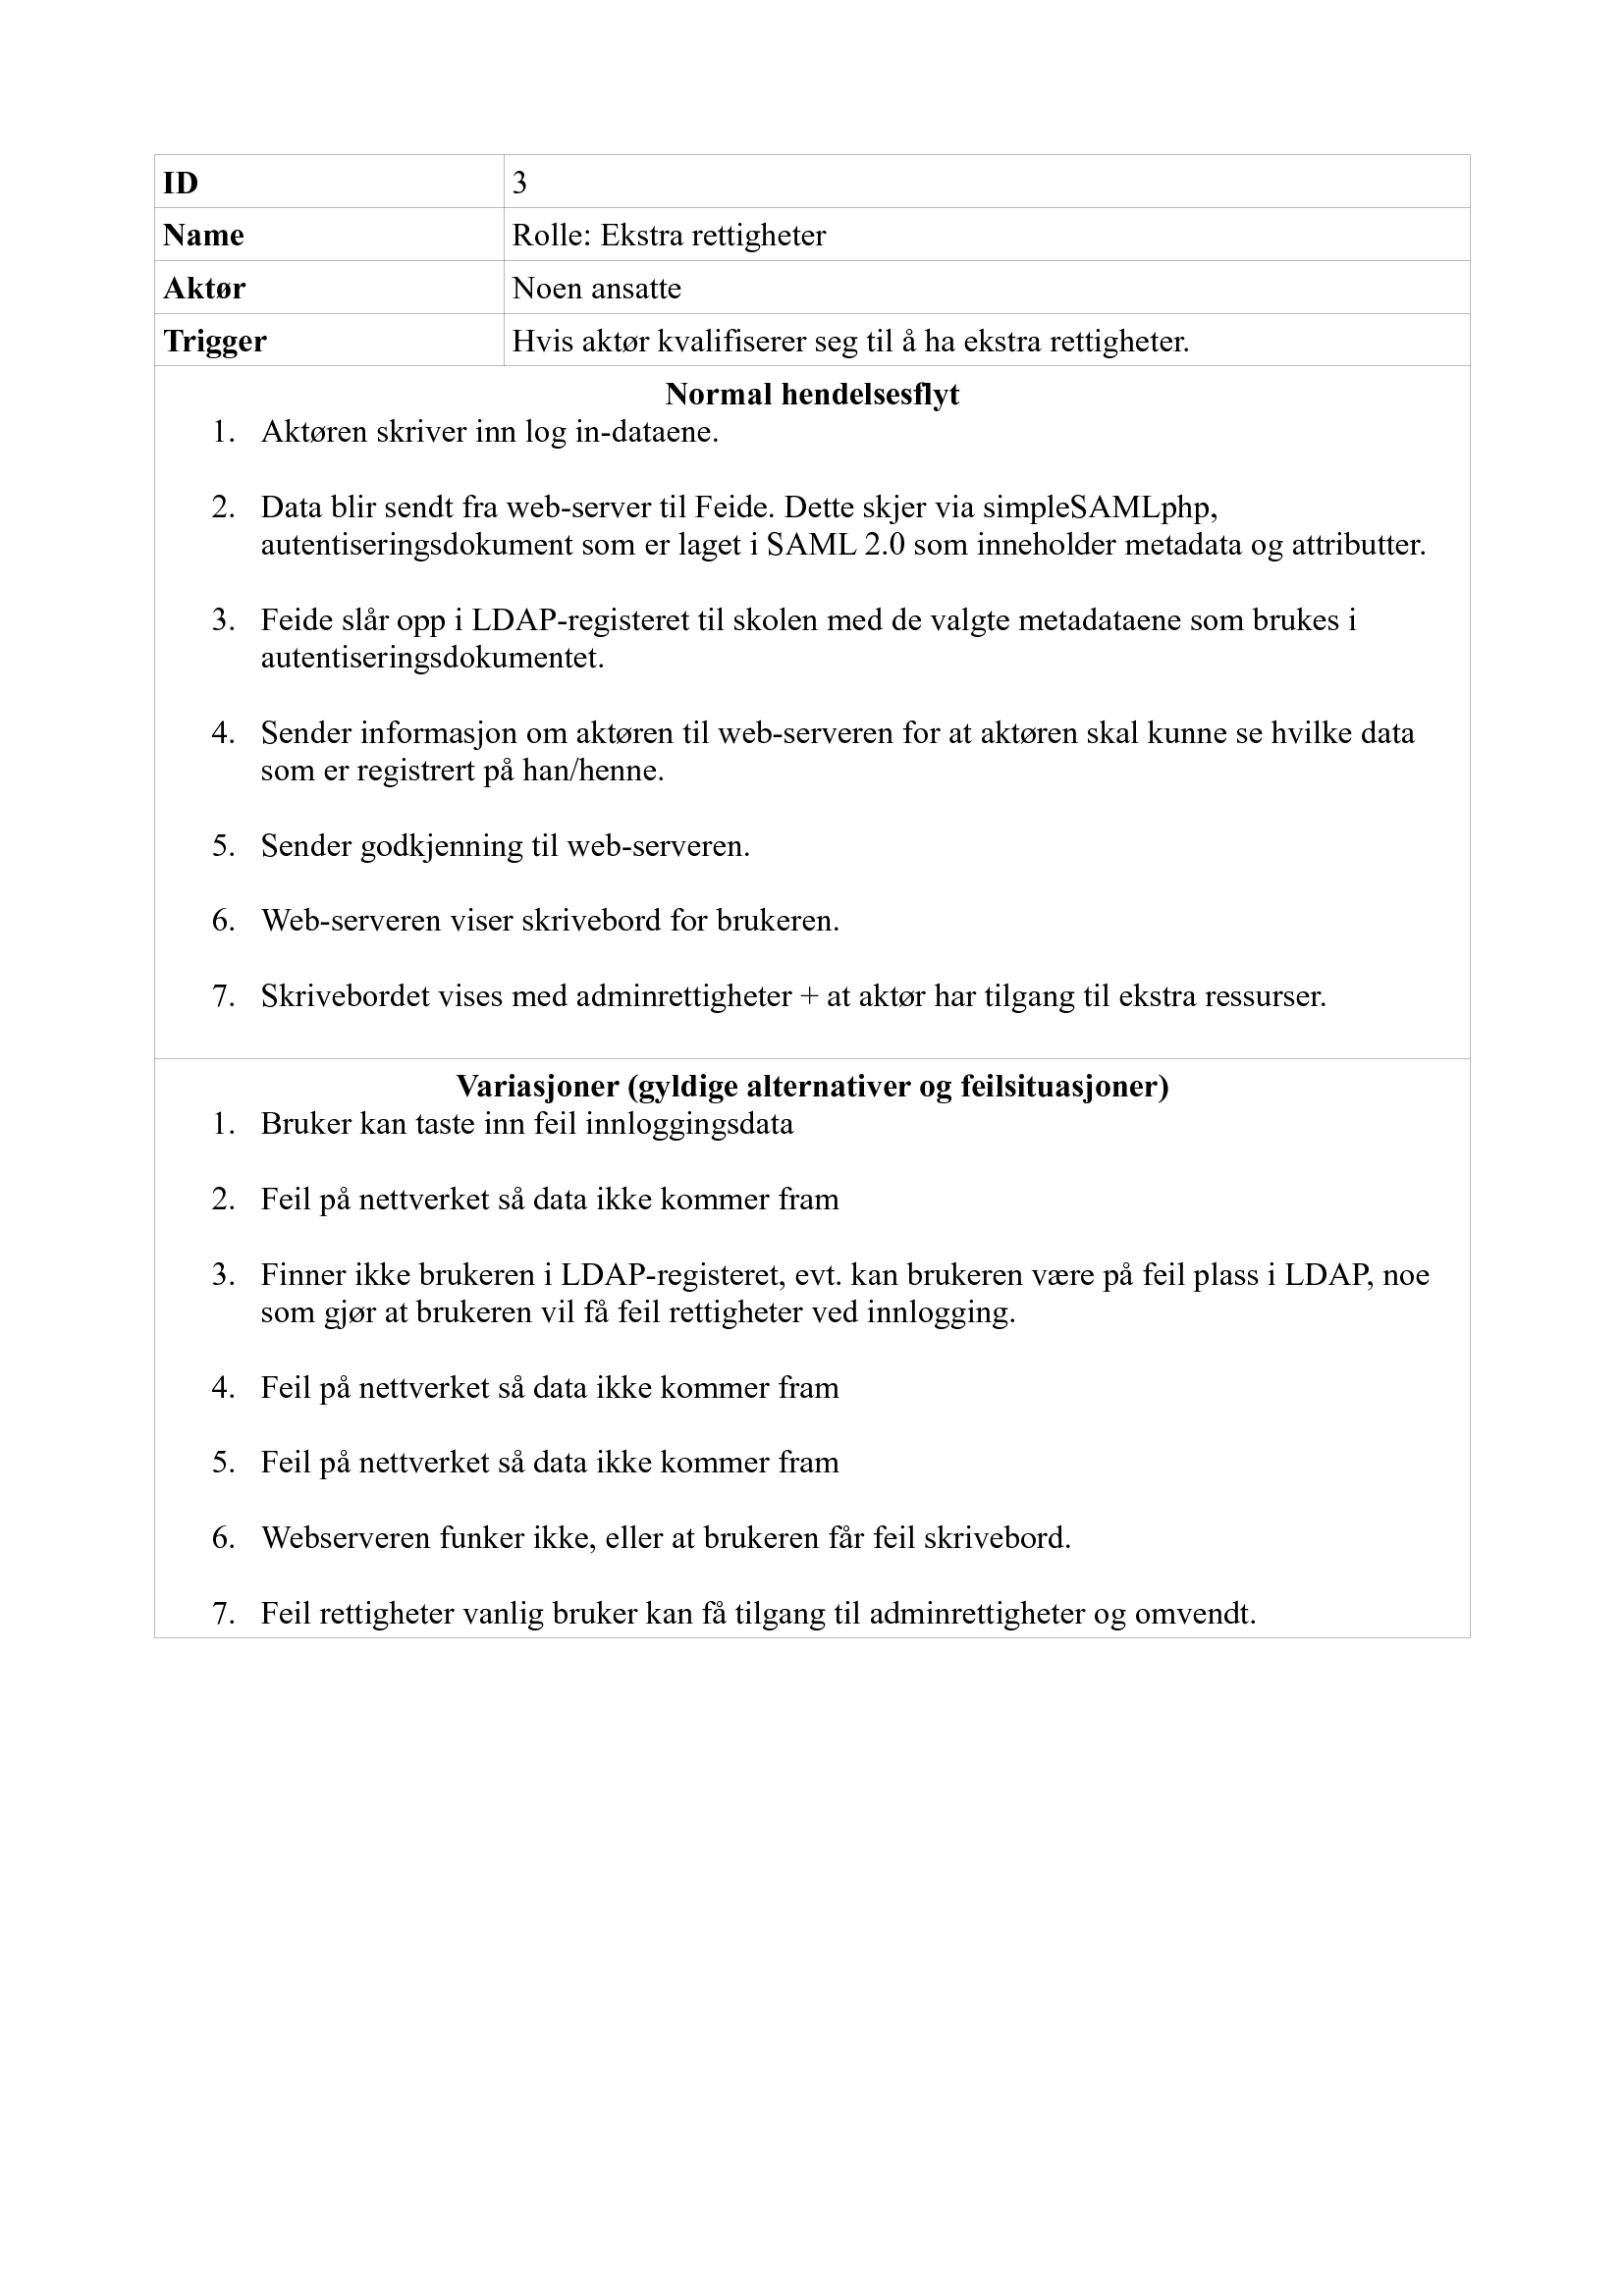
\includegraphics[height=280mm,width=150mm]{bilder/detaljert_usecase1}
	\caption{\label{fig:det_usecase1} Detaljert usecase}
\end{figure}
\newpage
\begin{figure}[H]
	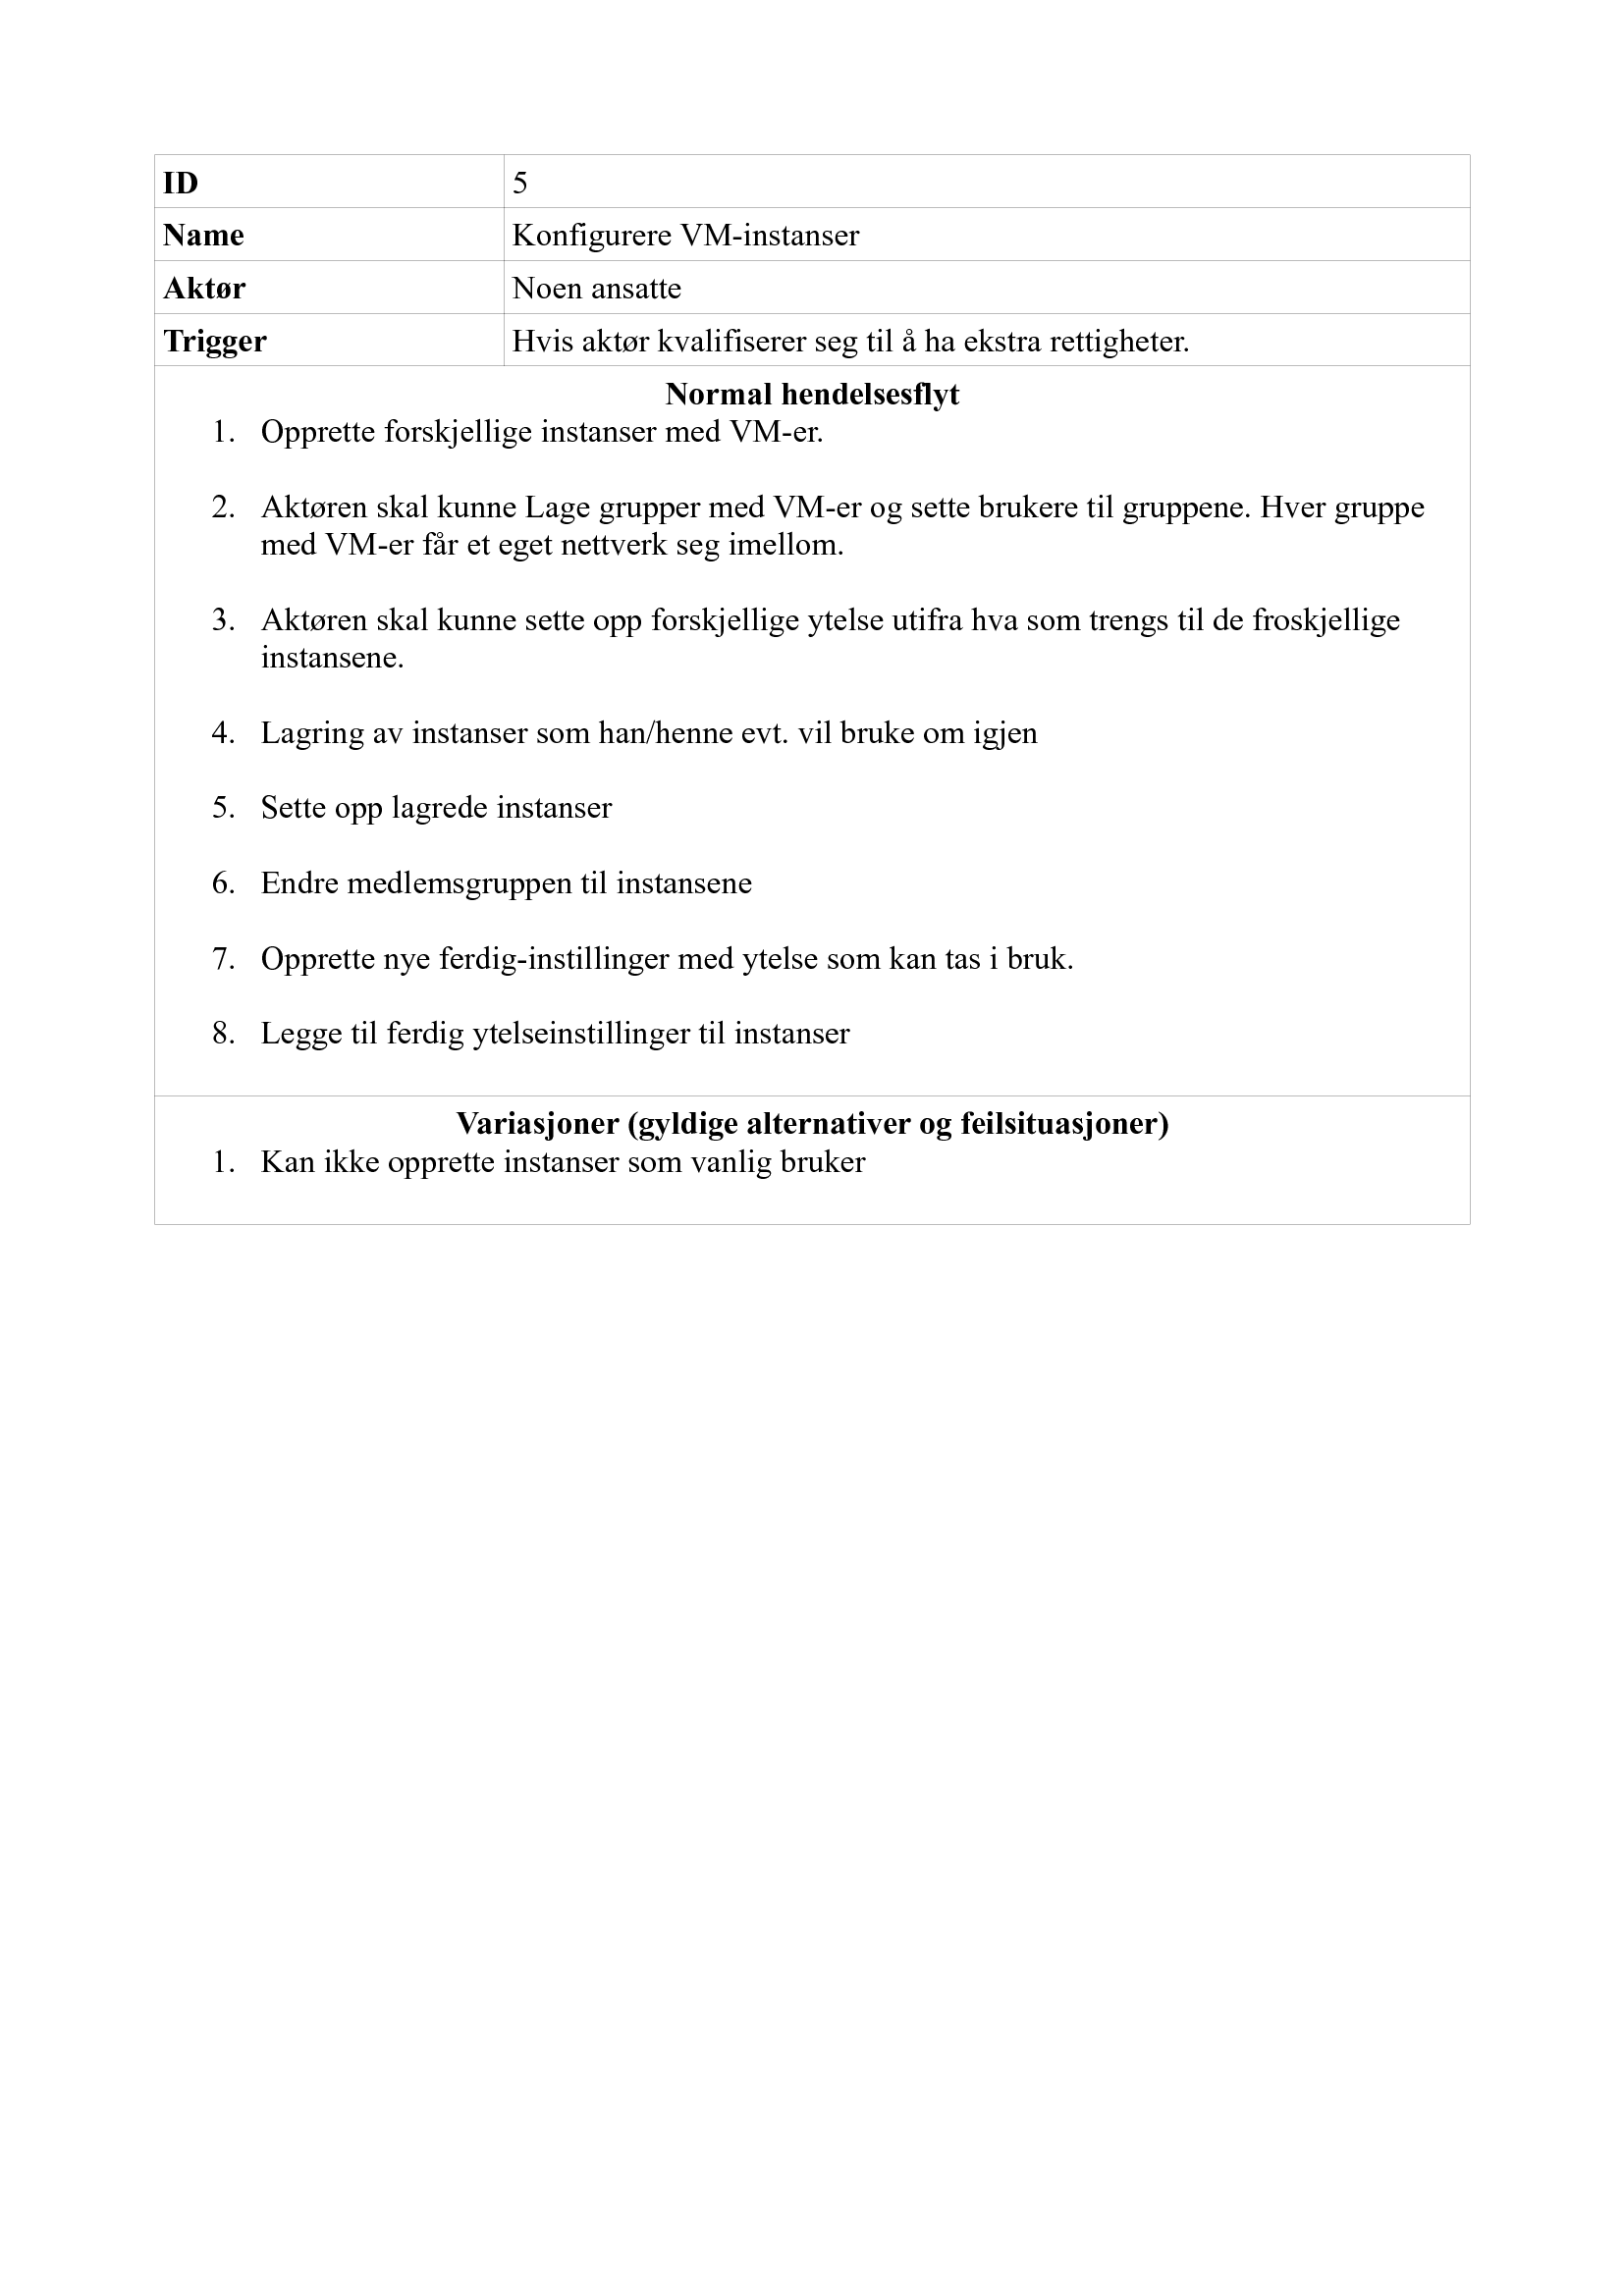
\includegraphics[height=280mm,width=150mm]{bilder/detaljert_usecase2}
	\caption{\label{fig:det_usecase2} Detaljert usecase}
\end{figure}
\newpage
\begin{figure}[H]
	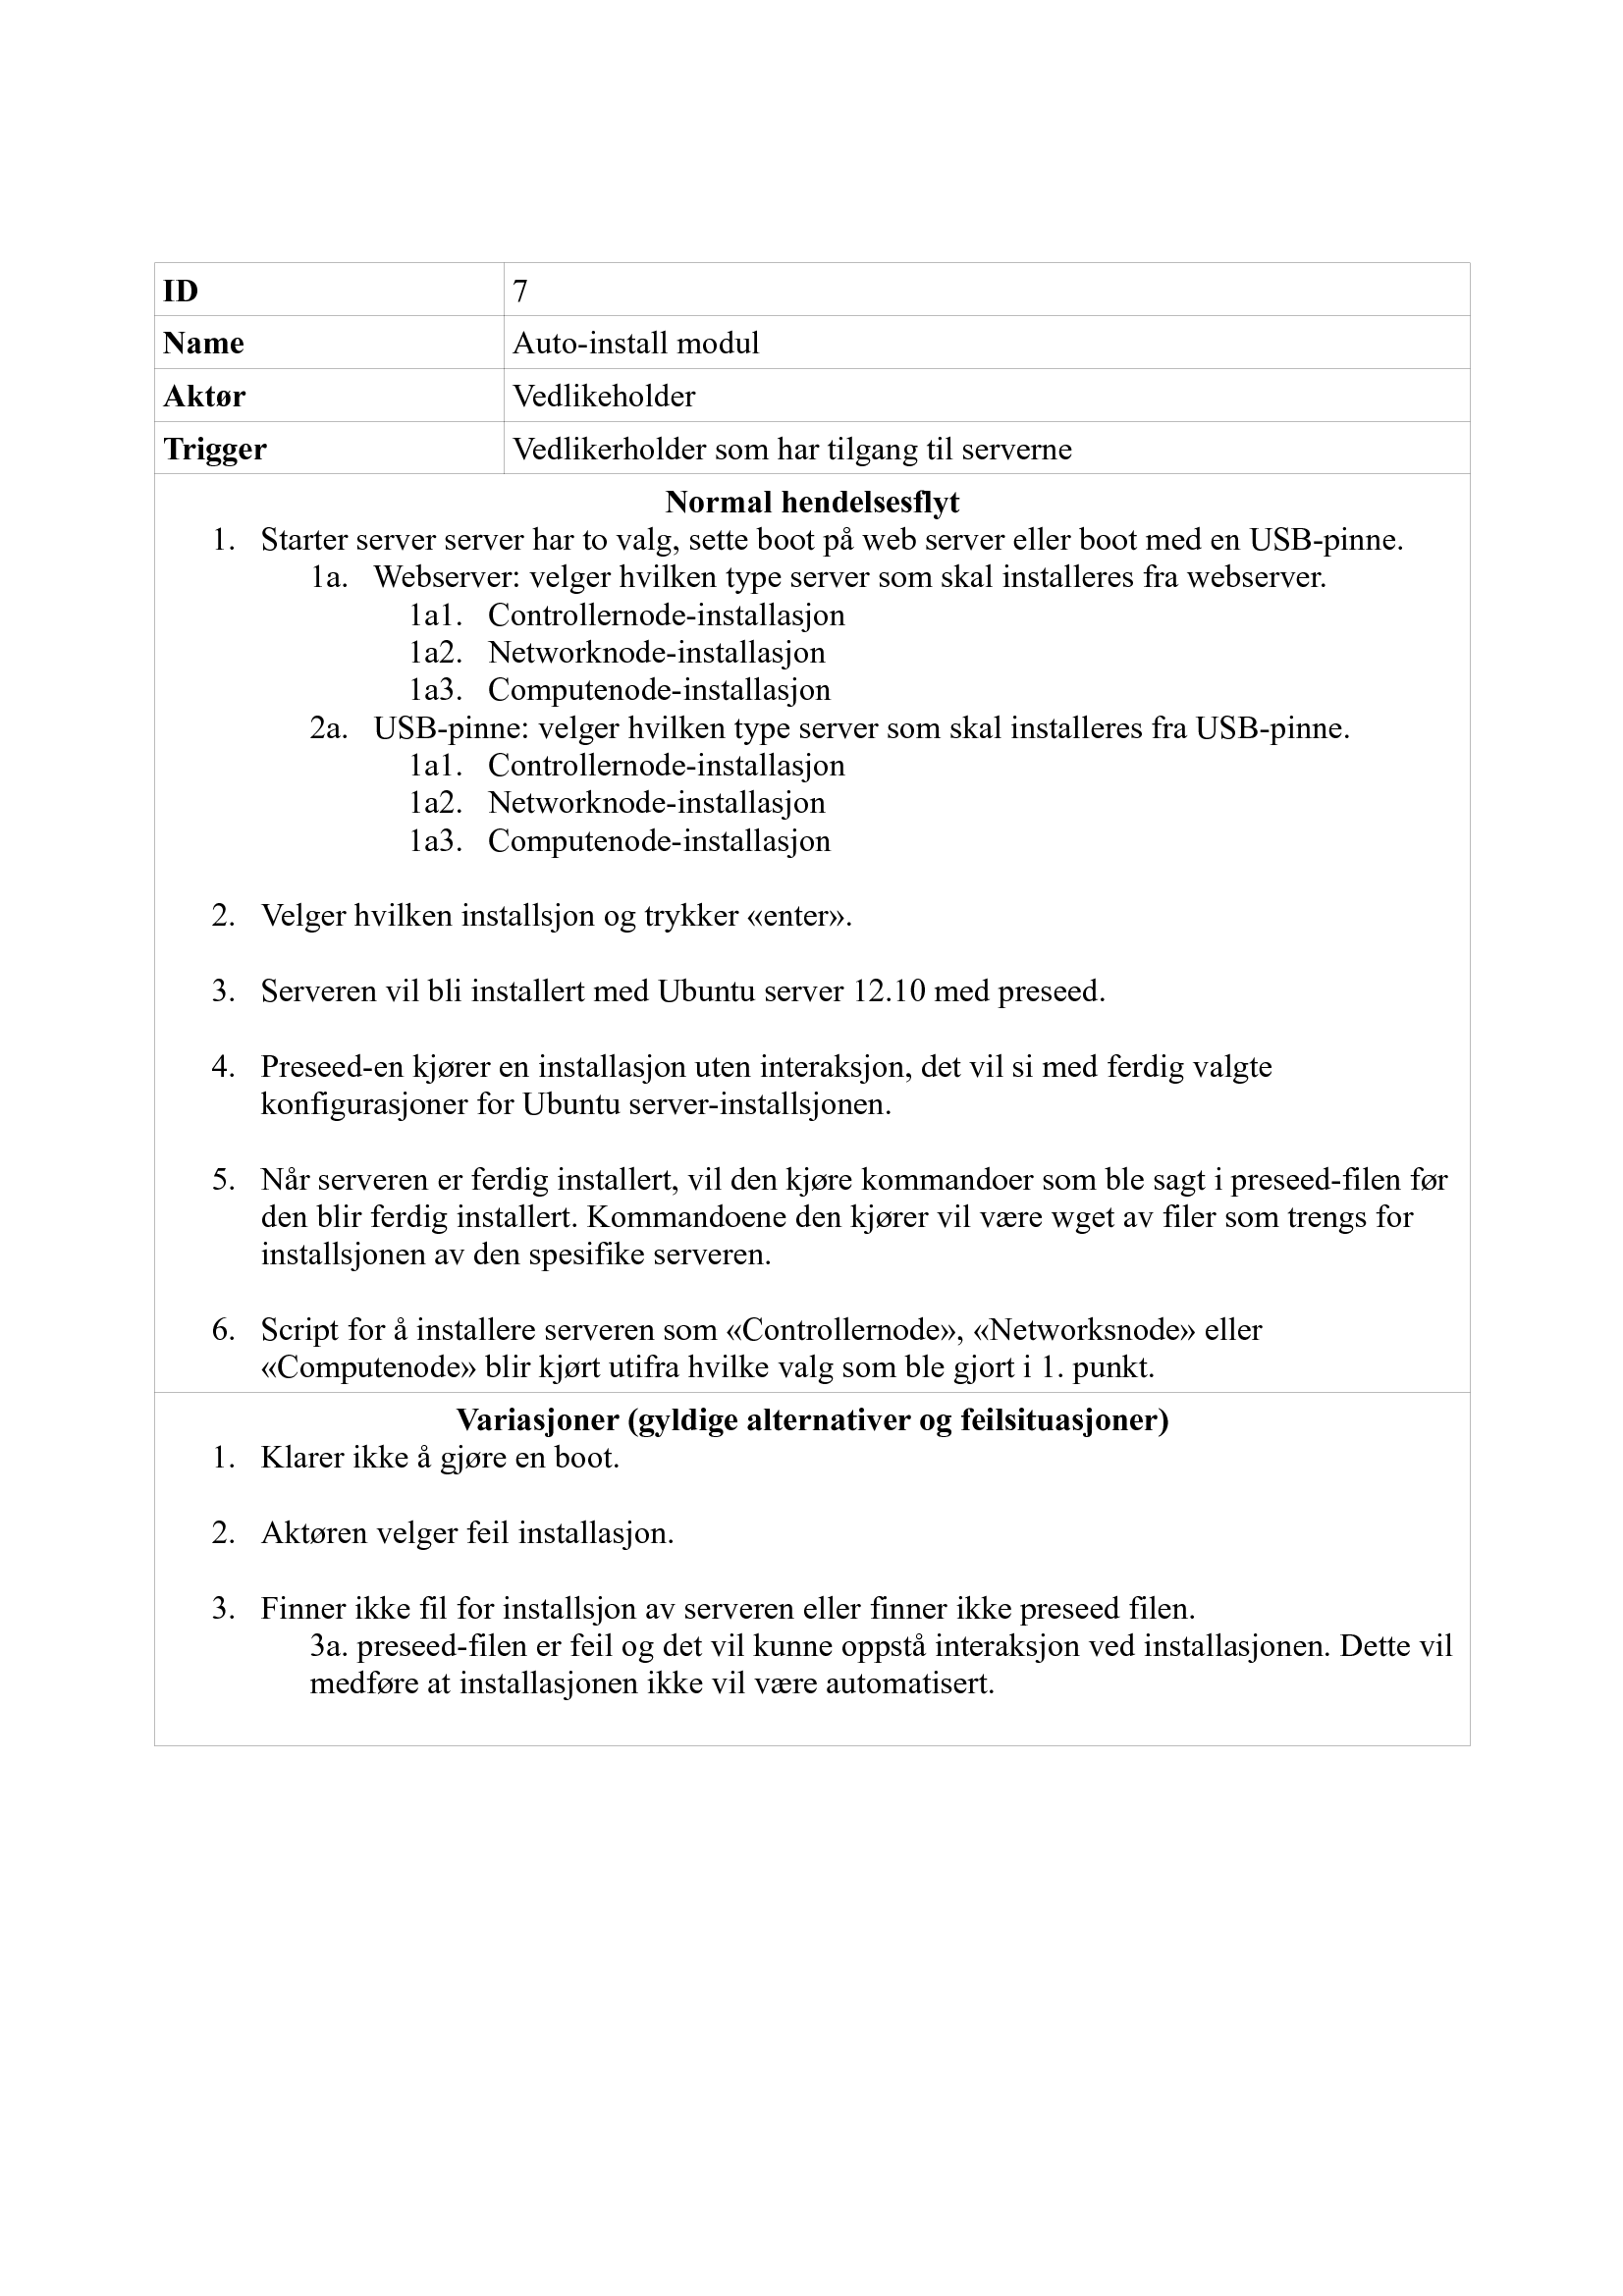
\includegraphics[height=280mm,width=150mm]{bilder/detaljert_usecase3}
    \caption{\label{fig:det_usecase3} Detaljert usecase}
\end{figure}

\clearpage
\subsection{Funksjon}
\begin{figure}[H]
      \center{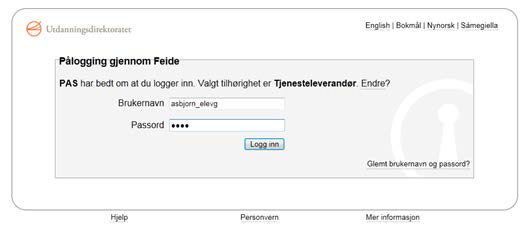
\includegraphics[height=50mm,width=100mm]{bilder/Palogging_via_Feide}}
      \caption{\label{fig:Pålogging_via_feide} Et eksempel på innlogging med feide}
\end{figure}
På figuren over kan du se hva som møter brukeren. På dette stadiet er det kun to datatyper, det er brukernavn og passord. Hendelserscenarioet er som figuren under.
\begin{figure}[H]
	\center{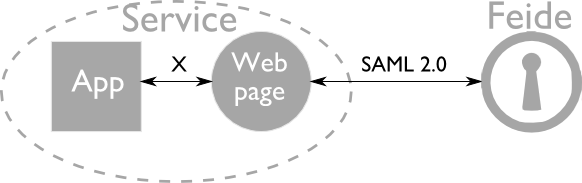
\includegraphics[scale=0.5]{bilder/innlogging-skjematisk}}
	\caption{\label{fig:Innlogging_skjematisk} Hvordan autentiseringen foregår}
\end{figure}
Webserveren er på kontrollernoden, Openstack-systemet er det vi kan referere til som appen på figuren over. Horizon er den som refereres til som “web page” på figuren, det er her vi skal lage innloggingsskjermen som vist på første figur.
\begin{description}
	\item{\tab •} Input - Brukernavn og passord fra brukeren. \\Skriver inn info, info-en blir sendt videre til Feide som er autentiseringsdatabase. Feide skjekker om bruker har tilgang og hvilken rolle brukeren har. Sender deretter info tilbake til “web page-en”.
	\item{\tab •} Output - Enten får brukeren at passord og brukernavn er feil, eller så kommer brukeren seg inn. Da vil brukergrensesnittet på Horizon vise seg for brukeren og brukeren kan lage, endre, slette og bruke VM-er utifra hvilken rolle/autentisering brukeren har.
\end{description}

\newpage
\subsection{Struktur og tverr-relasjoner}
\begin{figure}[H]
	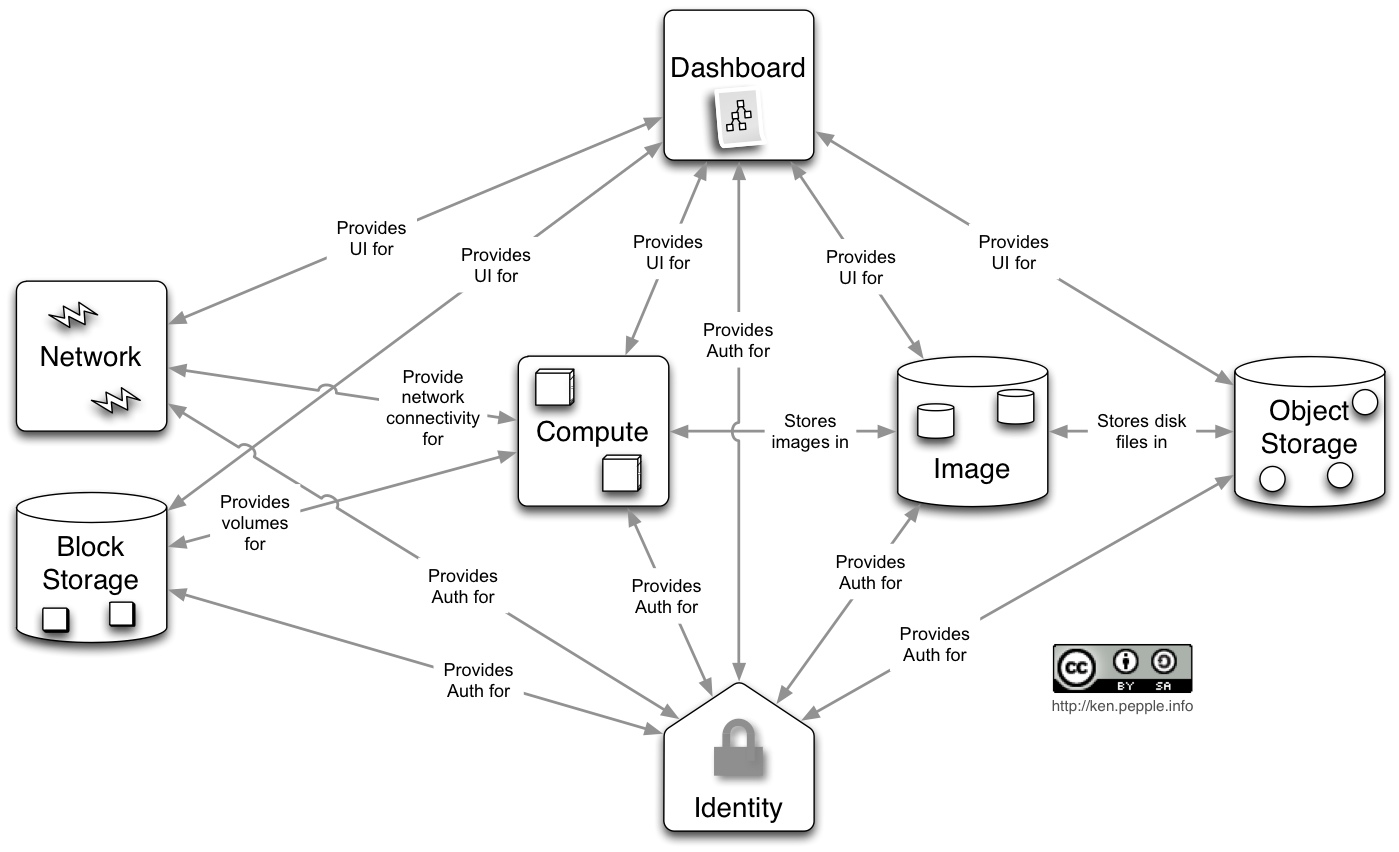
\includegraphics[width=150mm,height=100mm]{bilder/arkitektur_folsom}
	\caption{\label{fig:Struktur og tverr-relasjoner} Hvor går autentiseringstrafikken}
\end{figure}
Som du kan se på figuren over så går all autentifikasjon mellom dashboard og identity. Dashboard er Horizon og identity er Keystone. Horizon har kun autentisering mot keystone, det vil si at all vesentlig autentiseringsdata som keystone får går til Horizon. \newline \newline
Vi skjønner ut fra figuren, for at å autentisere mot FEIDE, så må vi vite hvilke data som kommer fra keystone. Når vi vet om de, så vet vi også hvilke data vi skal sende videre fra Horizon til FEIDE, utenom de obligatoriske attributtene (). 
%\section{Teoretisk grunnlag for Feide}
Feide er kunskapsdepartments løsning for sikker identifisering i utdanningssektoren. \\ \\
Feide er basert på konseptet føderert identidetishåntering. Dette vil si oppretting og autentisering av brukere skjer hos vertsorganisasjonene . Vertsorganisasjonene har også ansvar for administering av rettigheter, passord og personopplysninger. Tjenestetilbyder tar seg ikke av brukeradministrasjon, men administrerer rettigheter til tjenestene. \\ \\
\begin{description}
	\item[\tab •] Single Sign-On (SSO) er en måte å minske risiko for menneskelig feil. Brukeren vil da ha tilgang til flere program, tjenester eller datamaskiner ved bruk av samme brukernavn og passord.
	\item[\tab •] Single LogOut (SLO) er for å rydde opp. Hvis brukeren vil logge inn i en annen tjeneste så får brukeren oversikt over hvilke andre tjenester som man allerede er logget inn på. Uansett hvilken tjeneste og hvor man befinner seg så kan man logge ut av de andre tjenestene.
\end{description}
Føderert identifiseringshåndtering skaper et tillitsforhold mellom vertorganisasjonen og tjenesten. Tjenesten bruker opplysningnene som  vertsorganisisasjonen sitter med angående tilgangskontrollen og personidentifiseringen. \\
For at tjenestene fortsatt skal ha kontroll over de viktigste avgjørelsene så bruker Feide denne tilnærmingen:
\begin{description}
	\item[\tab •] Vertsorganisasjoner registrerer og autentiserer sine brukere.
	\item[\tab •] Tjenesteleverandører bestemmer egne tilgangsregler.
\end{description}

%\input{chapters/teoretisk grunnlag/openstack}
%\input{chapters/design}
%\input{chapters/gjennomføring}
%\input{chapters/driftsrutiner}
%\input{chapters/drøfting}
%\input{chapters/avslutning}

\bibliographystyle{unsrt}
\bibliography{main}

\appendix %after this line all chapters will have leters instead of numbers
\end{document}
